% das Papierformat zuerst
\documentclass[a4paper, 12pt, hidelinks]{report}
\usepackage{titlesec}

\titleformat{\chapter}[display]
  {\normalfont\bfseries}{}{0pt}{\Large}

\usepackage[pdftex]{graphicx}

\usepackage{fancyvrb}

\usepackage[left=25mm,right=20mm,top=25mm,bottom=25mm]{geometry}

\usepackage[utf8]{inputenc}
\usepackage[T1]{fontenc}

\usepackage[ngermanb]{babel}

\usepackage[hidelinks]{hyperref}
\usepackage{xcolor}
\usepackage{listings}
\colorlet{punct}{red!60!black}
\definecolor{background}{HTML}{EEEEEE}
\definecolor{delim}{RGB}{20,105,176}
\colorlet{numb}{magenta!60!black}
\lstdefinelanguage{json}{
    basicstyle=\normalfont\ttfamily,
    numbers=none,
    numberstyle=\scriptsize,
    stepnumber=1,
    numbersep=8pt,
    showstringspaces=false,
    breaklines=true,
    literate=
     *{0}{{{\color{numb}0}}}{1}
      {1}{{{\color{numb}1}}}{1}
      {2}{{{\color{numb}2}}}{1}
      {3}{{{\color{numb}3}}}{1}
      {4}{{{\color{numb}4}}}{1}
      {5}{{{\color{numb}5}}}{1}
      {6}{{{\color{numb}6}}}{1}
      {7}{{{\color{numb}7}}}{1}
      {8}{{{\color{numb}8}}}{1}
      {9}{{{\color{numb}9}}}{1}
      {:}{{{\color{punct}{:}}}}{1}
      {,}{{{\color{punct}{,}}}}{1}
      {\{}{{{\color{delim}{\{}}}}{1}
      {\}}{{{\color{delim}{\}}}}}{1}
      {[}{{{\color{delim}{[}}}}{1}
      {]}{{{\color{delim}{]}}}}{1},
}

% für bilder
\usepackage{graphicx}
% für floats (figures und so)
\usepackage{float}

% für Pfeile im Text Mode
\usepackage{textcomp}

\usepackage{subcaption}

\setlength{\parindent}{0pt}
\setlength{\parskip}{2mm}

\title{Augmented Reality auf mobilen Geräten}
\author{Mervyn McCreight, Tim Pauls}
\date{\today}

\newenvironment{mySourceCode}
{\begin{list}{}{\setlength{\leftmargin}{2em}}\item\scriptsize\bfseries}
{\end{list}}

% hier beginnt das Dokument
\begin{document}

% =======================================================================
% Titelseite


 % FH-Wedel Header.
\begin{figure}[h]
\centering

\includegraphics[width=350px]{graphics/fhwedel}
\label{fig:fhwedel}
\end{figure}




% nicht zu parsende Zeichen
\begin{verbatim}


\end{verbatim}

\begin{center}
\textbf{\LARGE{Augmented Reality auf mobilen Geräten}}\\
von Mervyn McCreight (Inf101368)\\
und Tim Pauls (Inf101369)

\end{center}

\begin{verbatim}
\end{verbatim}

\begin{center}
\textbf{\today}
\end{center}

\begin{verbatim}
\end{verbatim}

\begin{center}
\textbf{\large{Fachbereich: Informatik}}
\end{center}

\begin{verbatim}


\end{verbatim}

% Name && Adresse des Arbeitgebers
\begin{center}
\textbf{\large{Fachhochschule Wedel}} \\
\textbf{\large{Feldstraße 143, 22880 Wedel}} \\
\end{center}

% nicht zu parsende Zeichen
\begin{verbatim}


\end{verbatim}

% Arbeitsbezeichnung.
\begin{center}
\textbf{Projekt Virtuelle Realität und Simulation}
\end{center}

% nicht zu parsende Zeichen
\begin{verbatim}


\end{verbatim}

% Tabellarische Aufzählung der Dauer und der Betreuer.
\begin{flushleft}
\begin{tabular}{llll}

\textbf{betreut durch:}
& & & Marcus Riemer, B.Sc. \emph{(mri@fh-wedel.de)}\\
& & & Christian-Arved Bohn, Prof. Dr. \emph{(bo@fh-wedel.de)}\\

\end{tabular}
\end{flushleft}


\newpage


\newpage

% =======================================================================
% Inhaltsverzeichnis

\tableofcontents
\listoffigures
\newpage

% -----------------------------------------------------------------------
% Introduction

\section{Zielsetzung}
\chapter{Analyse}
Die Umsetzung des Projekts erforderte vorerst eine genauere Analyse des Projekts. Es ergibt sich, dass das Projekt logisch in verschiedene Teilaspekte unterteilbar ist.

\section{Augmented Reality auf einem mobilen Telefon}
Die grundlegende Überlegung ist, die Realität auf einem Handy in der Art darzustellen, dass diese nachträglich beliebig erweiterbar ist. Dies geschieht beispielsweise durch das Einblenden von nur virtuell existenten Objekten. Dadurch wird dem Benutzer eine Erweiterung der eigentlichen Realität vorgetäuscht.
Die Realität wird hierfür durch die Kamera des mobilen Gerätes aufgefangen und verarbeitet. Für die nachträgliche Bearbeitung reicht es jedoch nicht, das Bild der Kamera in einer Live-View wiederzugeben. Stattdessen muss eine 3D-Umgebung existieren, die es ermöglicht, nicht existente Objekte in das Bild einzufügen.

\begin{figure}[!h]
  \centering
    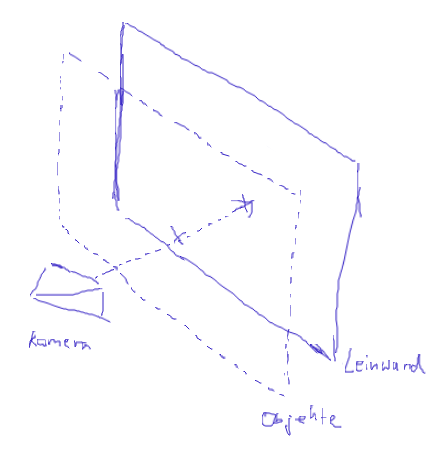
\includegraphics[width=6.5cm]{szene_skizze}
    \caption{Aufbau der AR-Szene}
    \label{fig:scene_sketch}
\end{figure}

Die Lösung ist eine simulierte Leinwand in einer 3D-Umgebung. Hierfür wird eine Fläche erstellt, die orthogonal zur Kamera steht. Diese Fläche wird mit dem Live-Bild der Kamera des mobilen Gerätes texturiert. Nun ist es möglich fremde Objekte in das Kamerabild einzufügen, indem man diese Objekte zwischen Leinwand und Kamera platziert.
Wichtig hierbei ist, dass die Leinwandfläche zu jeder Zeit orthogonal zur Blickrichtung der Kamera ist, da der Benutzer ansonsten den Abstand zwischen virtuellem Objekt und Leinwand sehen kann, wodurch die Illusion verloren geht. Ein weiteres Problem ist die Simulation von Tiefe auf diese Art und Weise. Die virtuellen Objekte stehen in der 3D-Umgebung in einem festen Abstand zur Leinwand. Wenn ein Objekt in der eigentlichen Realität nun weiter entfernt steht als ein anderes, muss die Tiefe durch eine Veränderung der Größe simuliert werden.

Um eine noch realistischere Darstellung der virtuellen Objekte zu ermöglichen, ist der Einsatz eines Virtual-Reality-Headsets möglich. Aufgrund der geringen Anschaffungskosten und der Kompatibilität zu vielen Mobilgeräten ist hierfür die Verwendung des Google Cardboard angedacht.

\section{Marker}
Ein genereller Ansatz zur Realisierung von Augmented Reality ist der Einsatz von Markern. Die Marker dienen als Stellvertreter von virtuellen Objekten in der Realität. Das Programm, welches Augmented Reality simulieren möchte, kann nun die Position und Orientierung der Marker durch Verarbeitung des Kamerabildes wahrnehmen, und virtuelle Objekte an dieser Stelle platzieren.
Eine wichtige Entscheidung ist die Wahl der Art des Markers. In diesem Projekt wurden sich für QR-Codes als Marker entschieden.
Bei dem QR-Code handelt es sich um ein weit verbreitetes Verfahren. Es existieren daher viele Bibliotheken, die das Verarbeiten von QR-Codes realisieren. Des weiteren ist das Erkennungs- und Leseverfahren für QR-Codes durch eine automatische Fehlerkorrektur sehr robust. Das ist wichtig, da die Auflösung des Kamerabildes für eine Live-Verarbeitung auf einem mobilen Gerät nicht zu hoch sein darf. Trotzdem müssen die Marker zuverlässig erkannt werden. Ein weiterer Vorteil ist, dass QR-Codes zusätzlich zur Position noch weitere Informationen im QR-Code selbst tragen können. Auf diese Weise ist es möglich, abhängig vom Marker verschiedene Inhalte einzublenden.

\section{Entwicklungsumgebung}
Bei der Wahl der Entwicklungsumgebung für mobile Anwendungen kann grundsätzlich zwischen zwei Ansätzen unterschieden werden. Zum einen kann nativ für eine Zielplattform entwickelt werden, zum anderen kann ein Framework oder eine Engine verwendet werden, die die Entwicklung abstrahiert. Beide Varianten bieten Vor- und Nachteile. Ausschlaggebende Kriterien sind die Effizienz, die Unterstützung für weitere externe Softwarekomponenten, die einfache Handhabung und mögliche Zielplattformen.

Ein Vorteil der nativen Entwicklung liegt in der Effizienz. Nur exakt die benötigten Komponenten sind in der finalen App vorhanden. Die Verwendung einer Engine führt häufig dazu, dass weitere, eigentlich ungenutzte, Abhängigkeiten die Dateigröße zusätzlich erhöhen, oder eine Auswirkung auf die Leistung haben.

Der große Vorteil in der Verwendung einer Engine liegt, darin, dass die Anwendung für unterschiedliche Zielplattformen veröffentlicht werden kann, ohne dass sie für jede Plattform von Grund auf neu entwickelt werden muss. Außerdem erleichtert eine Engine die Handhabung grafischer Funktionen, beispielsweise das Laden von 3D-Modellen und deren Positionierung im Raum.

Die Wahl der Entwicklungsumgebung fiel auf die 3D-Engine Unity. Zusätzlich zu den bereits genannten Vorteilen einer Engine unterstützt sie die Verwendung von Bibliotheken zur QR-Code-Erkennung (ZXing) und die Benutzung des VR-Headsets Google Cardboard. Zudem existieren viele Ressourcen, die die Einarbeitung in die Arbeit mit der Engine erleichtern.

\chapter{Tag der offenen Tür}

Die Entscheidung, mit Hilfe des Projektergebnisses eine Schnitzeljagd auf dem \glqq Tag der offenen Tür\grqq\ der FH-Wedel zu veranstalten, resultierte in verschiedene zusätzliche, auch innerhalb der Applikation logische, Anforderungen.
Der Ablauf der Schnitzeljagd wurde folgendermaßen entschieden:

\begin{itemize}
\item Es existieren QR-Codes, die Fragen beinhalten
\item Zu jeder Frage existiert ein QR-Code, der eine Münze beinhaltet
\item Die Münz-QR-Codes werden erst \glqq freigeschaltet\grqq\ , wenn ein Benutzer die zugehörige Frage korrekt beantwortet hat
\item Die Münzen müssen einmalig einsammelbar sein
\item Ein Benutzer hat die Schnitzeljagd gewonnen, wenn er alle Münzen eingesammelt hat
\end{itemize}
Folgende Anforderungen wurden für das Fragesystem formuliert:

\begin{itemize}
\item Die Fragen müssen dynamisch über ein Frontend ersichtlich und anlegbar sein
\item Die Applikation muss mit einem Fragen-Backend kommunizieren, um die Fragen zu erhalten und auswerten zu können
\end{itemize}

Hierfür müssen ein zusätzliches Front- und Backend entwickelt werden, dass die verschiedenen Fragen und Münzen verarbeitet, und dazu in der Lage ist für beide entsprechende QR-Codes zu generieren.
Zusätzlich dazu bietet das Frontend noch die Möglichkeit an, QR-Codes für Partikelsysteme zu generieren, die innerhalb der App an der Stelle des QR-Codes in die Umgebung simuliert werden können. Die veränderbaren Optionen beschränken sich zur Zeit auf die Start- und Zielfarbe der Partikel, dies lässt sich jedoch beliebig erweitern.

\section{Backend}
Das Backend wurde in PHP entwickelt. Die Entscheidung wurde getroffen, da der Server, auf dem das Backend laufen sollte, PHP bereits vorkonfiguriert hatte.

\subsection{Persistenz der Daten}
\label{sub:Persistenz}
Das Persistieren der verschiedenen Fragen und dazugehörigen Münzen, sowie der Partikelsysteme, geschieht direkt über das Dateisystem. Hierfür werden für die Fragen-/Münz- und Partikelsysteminformationen Dateien angelegt, die den entsprechenden Inhalt tragen. Die Informationen in den Dateien werden im JSON-Format hinterlegt.
Um die Speicherung zu strukturieren, wird automatisch folgendes Dateisystem aufgebaut, sobald eine Frage und/oder ein Partikelsystem angelegt wird:

\begin{verbatim}
<backend-root>
+-- question
|   +-- 1.json
+-- coin
|   +-- 1.json
+-- particle
|   +-- 1.json
\end{verbatim}

Das Beispiel zeigt das Dateisystem in einem Zustand mit einer angelegten Frage und einem angelegten Partikelsystem. Man sieht, dass für Fragen, Münzen und Partikelsysteme seperate Ordner anlegt werden. Zwischen Fragen und Münzen herrscht eine implizite 1:1 Verbindung. Daher ist eine Frage eindeutig über ihre ID zu einer Münze zuweisbar. Eine Münze besitzt daher immer die selbe ID wie ihre dazugehörige Frage. Die Partikelsysteme besitzen keine Verknüpfung zu den Fragen oder Münzen.

\subsection{API}
\label{subs:API}
Der lesende und schreibende Zugriff auf das Backend wurde über eine in PHP entwickelte RESTful-API realisiert. Die Implementierung befindet sich in der Datei \texttt{api.php}.
Die zugrundelegenden Datenstrukturen und Funktionen werden in der Datei \texttt{data.php} definiert. An dieser Stelle befindet sich die Logik der Serialisierung und der Speicherung im Dateisystem.
Die RESTful-API bietet folgende Zugriffs-URLs:

\begin{lstlisting}
POST:
/questions/         # Legt eine Frage mit den
                    # im POST-Request hinterlegten
                    # Daten an.
/particlesystems/   # Legt ein Partikelsystem mit den
                    # im POST-Request hinterlegten
                    # Daten an.

DELETE:
/questions/<id>     # Loescht die Frage mit der
                    # angegebenen ID.
/particlesystems/<id> # Loescht das Partikelsystem mit
                    # der angegebenen ID.

GET:
/questions/         # Liefert ein JSON mit allen aktuell
                    # existenten Fragen.
/questions/<id>     # Liefert ein JSON mit
                    # den Informationen zur Frage
                    # der entsprechenden ID.
/particlesystems/   # Liefert ein JSON mit allen aktuell
                    # existenten Partikelsystemen.
/particlesystems/<id> # Liefert ein JSON mit
                    # den Informationen zum Partikelsystem
                    # der entsprechenden ID.

/qrcodes/<id>       # Liefert ein JSON mit
                    # den Aufruf-URLs der
                    # Google-QRCode-API fuer Frage
                    # und Muenze mit der ID (200x200).
/qrcodesprint/<id>  # Liefert ein JSON mit
                    # den Aufruf-URLs der
                    # Google-QRCode-API fuer Frage
                    # und Muenze mit der ID (400x400).
/particleqrcode/<id>  # Liefert ein JSON mit
                    # den Aufruf-URLs der
                    # Google-QR-Code-API fuer
                    # das Partikelsystem mit der ID (200x200)
/particleqrcodeprint/<id>  # Liefert ein JSON mit
                    # den Aufruf-URLs der
                    # Google-QR-Code-API fuer
                    # das Partikelsystem mit der ID (400x400)

/questioncount/     # Gibt an, wie viele Fragen aktuell
                    # existieren.
\end{lstlisting}

\subsection{JSON-Format}
\label{sub:JSON-Format}
Es existieren verschiedene JSON-Serialisierungsformate für Fragen und QR-Code-Inhalte.

Das Format einer Frage ist folgendermaßen spezifiziert:
\begin{lstlisting}[language=JSON]
  {
    "question": "Fragetext",
    "answers": [
      "Antwort 1",
      "Antwort 2",
      "Antwort 3",
      "Antwort 4"
    ],
    "correctAnswer": 1,
    "id": 0,
    "type": 1
  }
\end{lstlisting}

Ein QR-Code-Inhalt wird verkürzt serialisiert, um den QR-Code so klein wie möglich zu halten. Dadurch beschleunigt sich die Echtzeitdekodierung. Anhand der ID wird die Verknüpfung zwischen Frage und Münze hergestellt.
\begin{lstlisting}[language=JSON]
  {
    "id": "1",
    "type": 1 // 0 = Muenze, 1 = Frage
  }
\end{lstlisting}

Für Partikelsysteme existiert eine weiteres JSON-Format, da für ein Partikelsystem zusätzlich zu seiner ID noch beliebig viele andere Zusatzdaten, die das Partikelsystem definieren, gespeichert werden müssen.
Bisher beschränken sich die konfigurierbaren Optionen auf die Start- und Zielfarbe der emitierten Partikel.

\begin{lstlisting}[language=JSON]
  {
    "id": "1",
    "type": 2 // Partikelsystem
    "startColor": "#000000" // Farben im HEX-Format.
    "endColor": "#000000" // Farben im HEX-Format.
  }
\end{lstlisting}

\section{Frontend}
Das Frontend besteht aus einer mit Twitter-Bootstrap entwickelten Seite. Das Frontend kommunziert hierbei über die RESTful-API mit dem Backend. Die Seite bietet einen Überblick über alle aktuell existierenden Fragen und Partikelsysteme, zusätzlich aller notwendigen Informationen (Fragetext, Antwortmöglichkeiten, korrekte Antwort, sowie Start- und Zielfarbe für Partikelsysteme).

Die Fragen und Partikelsysteme werden in seperaten Tabellen angezeigt. Diese sind hierbei nach ihrer ID sortiert. Ein Klick auf eine Zeile öffnet ein Modalfenster, über das es möglich ist eine Frage oder ein Partikelsystem zu editieren, in einem speziellen Format auszudrucken oder diese unwiderruflich zu löschen. Über einen Klick auf den \emph{Neue Frage anlegen}-Button oder den \emph{Neues Partikelsystem}-Button ist es möglich eine neue Frage oder ein neues Partikelsystem zu erstellen.

Die für die Funktionalität relevanten Funktionen, sofern sie nicht Bootstrap-intern sind, befinden sich in der Datei \texttt{overview.js}.

Zusätzlich zur nativen Twitter-Bootstrap Funktionalität, wurden zwei Open-Source Bootstrap-Addons verwendet. Hierbei handelt es sich zum einen um Bootstrap-Table\footnote{https://github.com/wenzhixin/bootstrap-table}, welches die Funktionalität von Tabellen in Twitter-Bootstrap erweitert, zum anderen um Bootstrap-Colorpicker\footnote{https://mjolnic.com/bootstrap-colorpicker/}, um in Bootstrap Komponenten einen HTML-Colorpicker zu integrieren.

\chapter{App}
\section{Unity}
\label{sec:Unity}
Projekte in Unity setzen sich aus Szenen zusammen, in denen Objekte platziert sind. Diese Objekte besitzen Eigenschaften, die direkt im Unity-Editor gesetzt werden können, z.B. Position oder Material. Zusätzlich können die Objekte mit Skripten verbunden werden, die ihr Verhalten beeinflussen.

\subsection{Verzeichnisstruktur}
\label{sec:Verzeichnisstruktur}
Im Verzeichnis Assets innerhalb der Projekt-Root befinden sich im Wesentlichen alle externen Dateien, die für das Projekt benötigt werden. Es existieren folgende Unterverzeichnisse:

\begin{itemize}
  \item \_Scenes -- enthält die Szenen-Dateien der App, die im Unity-Editor bearbeitet werden können
  \item Audio -- enthält Sounddateien (Frage richtig beantwortet, Frage falsch beantwortet, Münze eingesammelt)
  \item Cardboard -- Verzeichnis des Cardboard SDK
  \item Font -- enthält den in der App verwendeten Font (Ubuntu)
  \item Graphics -- enthält das FH Wedel Logo zur Verwendung als App-Logo, sowie zur Verwendung als Normal-Map auf der Münze
  \item Materials -- enthält verwendete Texturen (für die Münze und die Ka\-me\-ra\-bild-Ebene)
  \item Plugins -- enthält verwendete Plugins; sowohl von Unity direkt (Android), als auch von uns (ZXing)
  \item Prefabs -- enthält zur mehrfachen  Verwendung erstellte Bausteine (der in der App verwendete Button)
  \item Resources -- enthält Ressourcen, die zur Laufzeit des Programms dynamisch geladen werden (die Münze und das Partikelsystem)
  \item Scripts -- enthält die verwendeten C\#-Dateien
\end{itemize}

\subsection{Szenen}
\label{sec:Szenen}
Die App besitzt vier Szenen:

\begin{enumerate}
  \item MainMenuScene
  \item HelpScene
  \item CameraScene
  \item QuestionScene
\end{enumerate}

Im Folgenden wird kurz erläutert welchen Zweck die Szenen dienen, welche Objekte sie enthalten und mit welchen Skripten sie zusammenhängen.

\subsubsection{MainMenuScene}
\label{subs:MainMenuScene}
Diese Szene dient als Einstiegspunkt der App und stellt das Hauptmenü dar. Wichtige Elemente der Szene sind das Canvas-Objekt, das drei Text-Objekte (für den Titel und die Anzeige des Spielfortschritts), sowie drei Buttons (Wechsel zur Kamera, Hilfe und Beenden) enhält. Das Canvas-Objekt ist mit dem Skript \texttt{MainMenuUi.cs} verknüpft, das die Liste aller Fragen aus der API lädt und die Interaktion mit den Buttons behandelt.

\subsubsection{HelpScene}
\label{subs:HelpScene}
Die HelpScene dient der Anzeige eines kurzen Erläuterungstextes innerhalb der App. Sie ähnelt dem Aufbau der MainMenuScene mit einem Canvas, in dem Text- und Button-Objekte liegen. Der Canvas ist mit dem Skript \texttt{HelpUi.cs} verknüpft.

\subsubsection{CameraScene}
\label{subs:CameraScene}
Die CameraScene ist dafür zuständig das aktuelle Kamerabild anzuzeigen und eventuell vorhandene QR-Codes im Bild zu erkennen und zu behandeln. Die Behandlung erfolgt entweder durch einen Szenenwechsel zur QuestionScene, oder durch das Anzeigen einer Münze oder eines Partikelsystems vor der Position des QR-Codes. Außerdem können in dieser Szene kurze Nachrichten an den Nutzer in Form einer Toast-Message angezeigt werden.

Die Szene enthält immer eine Ebene im 3D-Raum, auf die das Kamerabild projiziert wird, sowie einen Canvas mit einem Toast-Objekt. Weitere Objekte, wie die Münze oder das Partikelsystem, die sich vor den QR-Codes befinden, werden im Code erzeugt.

Da zu Beginn der Entwicklung der Fokus mehr auf der Verwendung des Google Cardboard lag, befindet sich die Ebene in der Objektstruktur direkt unterhalb der \emph{Main Camera} im \emph{Head} des \emph{CardboardMain}-Objekts. Somit bewegt sich die Ebene stets mit dem Kopf des Nutzers mit und das Kamerabild befindet sich immer direkt vor der Engine-Kamera.

Die gesamte Logik der CameraScene wird durch \texttt{CameraScript.cs} gehandhabt, welches mit der Kamerabild-Ebene verknüpft ist.

\subsubsection{QuestionScene}
\label{subs:QuestionScene}
Die QuestionScene stellt die zum gescannten QR-Code passende Frage, sowie deren Antwortmöglichkeiten dar. Die Reihenfolge der Antworten wird bei jedem Aufruf einer Frage zufällig durchgemischt. Der Nutzer kann durch Tippen eine Antwort auswählen und erhält ein visuelles und akustisches Feedback, ob seine Wahl korrekt war. Auch diese Szene basiert im Kern auf einem Canvas, das Text-Objekte und Buttons enthält und mit dem Skript \texttt{QuestionUi.cs} verknüpft ist.

\section{Code-Dokumentation}
\subsection{QR-Code-Erkennung}
Über die Unity-Klasse \texttt{WebCamTexture} wird auf das aktuelle Kamerabild zugegriffen. Dieser Zugriff ist, wie bei anderen Unity-APIs auch, nur vom Main-Thread aus erlaubt. Um das Durchsuchen des Bilds von der Darstellung der App loszukoppeln erfolgt die QR-Code-Erkennung auf einem separaten Thread. Die Pixeldaten der Kamera werden in der \texttt{Update}-Methode des \texttt{CameraScript} (also einmal pro Frame) in einem Feld gespeichert. Der Thread liest kontinuierlich die Daten aus diesem Feld aus und versucht QR-Codes im Bild zu erkennen. Hierbei kommt die Bibliothek \emph{ZXing} zum Einsatz. Das Ergebnis einer Erkennung besteht aus den Pixelkoordinaten der \emph{Points of Interest}, sowie einer Binärpixelmatrix des QR-Codes selbst, anhand der der Inhalt dekodiert werden kann. Schließlich wird eine Sammlung mit erkannten QR-Codes mit den Ergebnissen aktualisiert (siehe \texttt{QrCodeCollection} und \texttt{QrCodeData}).

\subsection{QR-Code-Verarbeitung}
Ist bisher noch kein QR-Code im Sichtfeld der Kamera, wird der QR-Code im Anschluss an die Erkennung dekodiert. Basierend auf den enthaltenen Daten soll ein entsprechendes 3D-Objekt erzeugt und dargestellt, oder die Szene gewechselt werden. Als Orientierungspunkt dient der Mittelpunkt des QR-Codes. Dieser muss zunächst aus den \emph{Points of Interest} errechnet werden.

\begin{figure}[!h]
  \centering
    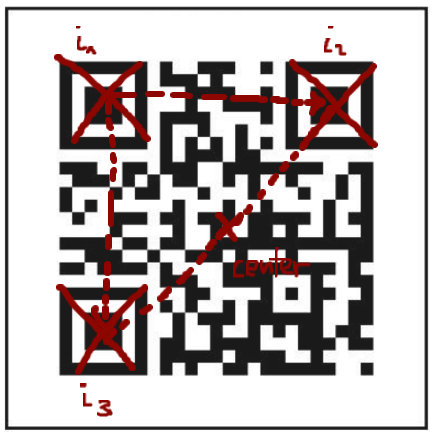
\includegraphics[width=5cm]{graphics/qr_code_center}
    \caption{Mittelpunktberechnung eines QR-Codes anhand seiner POIs}
    \label{fig:qr_center}
\end{figure}

Die Verbindungslinie der beiden \emph{Points of Interest}, deren Distanz zueinander am größten ist, bildet die Diagonale. Der Mittelpunkt dieser Diagonale ist das Zentrum des QR-Codes.

Das Programm befindet sich zu dem Zeitpunkt der QR-Code-Verarbeitung nicht in dem Unity-Main-Thread. Daher kann nicht direkt ein Objekt angelegt werden. An dieser Stelle wird ein entsprechend markiertes \texttt{QrCodeData}-Objekt in die \texttt{QrCodeCollection} eingefügt. Die eigentliche Erzeugung des 3D-Objekts erfolgt in der \texttt{Update}-Methode des \texttt{CameraScript}s und somit auf dem Unity-Main-Thread.

Ist bereits ein QR-Code im Sichtfeld, wird seine Position anhand der neu erkannten Positiondaten aktualisiert. Auf Basis der neu erkannten Position wird eine Zielposition für das \texttt{QrCodeData}-Objekt berechnet.

\begin{figure}[!h]
  \centering
    \begin{subfigure}{0.42\textwidth}
      \centering
        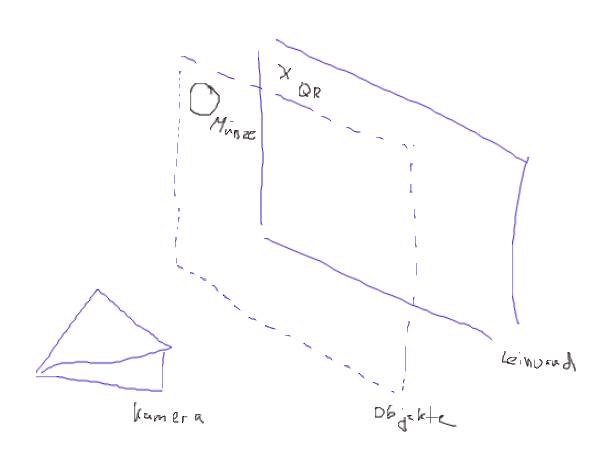
\includegraphics[width=\textwidth]{graphics/position_skizze_falsch}
      \caption{Naiver Ansatz}
    \end{subfigure}%
    \begin{subfigure}{0.42\textwidth}
      \centering
        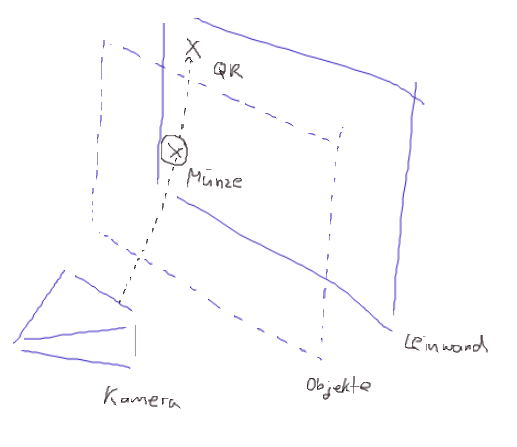
\includegraphics[width=\textwidth]{graphics/position_skizze_richtig}
      \caption{Korrekter Ansatz}
    \end{subfigure}
    \caption{Positionsberechnung der 3D-Objekte anhand der Markerposition}
    \label{fig:position_sketch}
\end{figure}

Bei der Berechnung der Positionierung muss beachtet werden, dass sich das Objekt nicht direkt auf der Leinwand, sondern auf einer gedachten Ebene davor befindet. Um zu gewährleisten, dass ein eingeblendetes Objekt korrekt vor dem QR-Code angezeigt wird, darf nicht die erkannte Position des QR-Codes übernommen werden. Stattdessen muss ein Strahl vom Augpunkt zur Position des QR-Codes auf der Leinwand geschossen werden. Der Schnittpunkt des Strahls mit der Objekt-Ebene ist die korrekte Position des 3D-Objekts.

Die Anpassung der Position zwischen aktueller und Zielposition wird in jedem Frame linear interpoliert, damit die Bewegung des 3D-Objekts flüssiger dargestellt wird. Leicht ungenaue Positionserkennung und eine handgeführte Kamera werden dadurch ausgeglichen.


\section{Google Play}
Wie eine App im Google Play Store veröffentlicht wird kann hier nachgelesen werden: http://developer.android.com/distribute/googleplay/start.html.

Zu beachten ist, dass man aus Unity ein \textbf{signiertes} APK für den Upload im Play Store exportiert. Dafür muss in Unity unter \emph{Edit \textrightarrow\ Project Settings \textrightarrow\ Player \textrightarrow\ Android Tab \textrightarrow\ Publishing Settings} ein existierender Keystore eingetragen oder ein neuer angelegt werden. Anschließend kann über \emph{File \textrightarrow\ Build Settings} ein Android Build gestartet werden, der den gewählten Keystore und Alias verwendet, um das Package zu signieren. Der Keystore muss unbedingt sicher aufbewahrt werden, da Updates für eine einmal veröffentlichte App nur mit dem selben Keystore und Alias erneut signiert werden können. Geht der Keystore verloren, muss auch die App im Play Store neu angelegt werden (mehr Details hier: http://developer.android.com/tools/publishing/app-signing.html\#secure-key).



% ===================================================0
% End of Document
\end{document}
